\section{Lee-Liu Algorithm}
\subsection{Overview of algorithm}
As previously mentioned, our research project and UPPAAL model are based on the work by Yang Liu and Kiju Lee \parencite{AlgorithmPaper}. The article describes an algorithm for reaching a consensus in a decision-making process between an arbitrarily large swarm of independent, autonomous robots or agents that work together to accomplish some task. The algorithm was selected because it poses an interesting challenge in modeling the communication between agents, and because it suggests a number of experimentally decided metrics for how the algorithm should work. These metrics are useful for us to compare against our own model implementation.

The authors establish the following constraints on the algorithm (p. 3):
\begin{itemize}
\item Individual robots are primitive with limited sensing, communication, and processing capabilities.
\item Communication in the swarm is local; each robot can communicate only with nearby robots within the communication range. Robots within range will be referred to as neighbors for the rest of this report.
\item Robots have no temporal memory (i.e. no log of history data) and function like finite state machines.
\end{itemize}
We also note three assumptions:
\begin{itemize}
    \item The topology of the network will not change during the decision-making process.
    \item Robots have perfect and consistent communication among their neighbors.
    \item Robots are assumed to be somewhat globally synchronized, as the network is evaluated in terms of iterations. 
\end{itemize}

In summary, the algorithm works as follows:
\begin{itemize}
    \item There are $m$ robots, identified by their index in the set $R$. The set of possible decisions, \textbf{Q}, contains the indices for \textit{n} different choices. 
    \item Each individual robot is initialized with a distribution of preferences for each possible choice, given as a probability mass function $P_k$ for robot $R_k$. Each robot exhibits a decision, which is the choice it has the highest preference towards. For example, if $n = 3$, $R_k$ may have the set of preferences $\{P_k(1) = 0.25, P_k(2) = 0.5, P_k(3) = 0.25\}$, and it will exhibit a decision of choice 2.
    \item A robot has a connection group, \textit{C}, which consists of all of its neighbors. The robot knows the IDs and preference distributions of its neighbours. 
    \item A robot has a consensus group, \textit{D}, which consists of the largest connected component of robots that share the same dominant preference. See figure 1 below. A robot knows the IDs, but not the preference distributions, of the members in its consensus group. 
    \item A robot continuously updates its preference distribution by exchanging information with its neighbours. A robot will update its preferences to align with the predominant opinion among its neighbours, especially if their consensus groups are large.
    \item As the algorithm runs, the robots will become more certain in their decisions and stabilize their preference distributions, as long as nothing new is introduced in the network.
    \item When all robots share the same dominant preference, the algorithm terminates.
\end{itemize}

\begin{figure}[H]
    \centering
    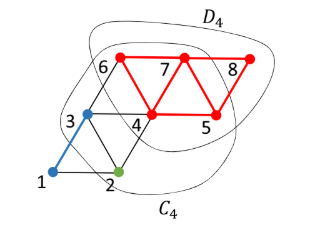
\includegraphics[width=0.5\linewidth]{pictures/Lee-Liu figure.png}
    \caption{"A network showing \(R_4\)'s local consensus group \(D_4\)
    and local connection group \(C_4\)" \parencite[Fig. 2]{AlgorithmPaper}.}
    \label{fig:ConsensusGroupsFromArticle}
\end{figure}

For a detailed explanation of the algorithm, we refer the reader to the original article \parencite{AlgorithmPaper}.
%For a more thorough explanation of the algorithm, the math and for an explicit use of the introduced formulas, see the original algorithm article and our UPPAAL implementation details.

\subsubsection{Interesting facets of the algorithm in modeling}

Apart from these assumptions that were explicitly stated in the original article, it is mentioned that the individual robot updates the members of its local consensus group. However, the provided explanation does not exhaustively address the issue that arises when one such change happens at a critical node in the local network of the consensus group. This, however, has become apparent as a result of our work in modelling the algorithm. 

To address this shortcoming, we present two different solutions: One makes use of our custom implementation of the Depth-first search algorithm\footnote{\url{(https://en.wikipedia.org/wiki/Depth-first_search)}} in UPPAAL to scan a global structure of the existing consensus groups, and thus finding their size, during every exchange of information between the individual robots. This approach adheres to the assumption of perfect local knowledge of the agents, but fails to adhere to the constraint of local communication. To rectify this issue, we present a second solution that follows more realistically the intended scenario - that the individual robots are indeed only able to communicate with their neighbours, and as such must use other means to address the predicament of figuring out the size of its local consensus group at any given time. This comes at a cost in convergence time, which we will discuss in later sections.
The authors of the article specifically state that interesting new avenues of research for the algorithm includes improvements to the discovery and updating of local consensus groups, including possible changes to the algorithm. This notion has also informed our decision in developing the previously mentioned UPPAAL models.

\subsubsection{Expected behaviour and results}
Lee and Liu present a number of different expected outcomes of their algorithm, as well as some ideal and anticipated behaviour under different circumstances based on both theoretical estimations and simulations done in a python script. These expectations are important benchmarks for us to compare against our own findings in our UPPAAL implementation of the algorithm. Here, we list some of the findings that we will discuss further in the results section of this paper.
\begin{enumerate}
    \item The network always reaches a consensus.
\end{enumerate}
This property of the algorithm serves as an important sanity check for us to determine that the model acts as intended. It is also the first property that we will check with our modeling tool.
\begin{enumerate}
    \setcounter{enumi}{1}
    \item The convergence rate is moderately correlated with network dependency.
\end{enumerate}
Network dependency is a term coined by Lee and Liu in the research article. Network dependency denotes the importance of the most critical node on maintaining the network connectivity \parencite[page 6]{AlgorithmPaper}. To facilitate testing the properties, we have coded a model generation tool in python that can also determine the network dependency value of the networks we use in simulation. We elaborate on this in section \ref{subsec:GG}.
\begin{enumerate}
    \setcounter{enumi}{2}
    \item The number of iterations needed to reach consensus is positively correlated with network size \textit{m} and the number of decisions \textit{n}.
\end{enumerate}
Larger networks and networks with a larger decision space take longer to correlate. We expect to see similar behaviour in our UPPAAL implementation.
Next follow a number of tests that we will try to replicate in our model, although the results are somewhat difficult to exactly reproduce, as they are based on randomly generated networks and their specific topologies.
\begin{enumerate}
    \setcounter{enumi}{3}
    \item The network converges significantly faster when seeded. The size of the seeding group and its placement in the network significantly affects this property.
\end{enumerate}
With 10 seed robots, a network of a 100 robots exhibits a 53\% convergence rate towards the dominant opinion of the seed robots. We will create similar trials to see if we can observe similar behaviour in our model.

\subsection{Graph Generation}
\label{subsec:GG}
For the purposes of testing and verifying their algorithm, Lee and Liu use a number of randomly generated networks. These networks have certain characteristics and properties that are relevant for the metrics of the algorithm. First, the networks are generated with a specific amount of robots \textit{m} and opinions \textit{n}. Second, all robots in the network have a maximum of 6 neighbours. This forms the equilateral triangle grids that is shown in the figures of the algorithm paper. Lastly, these graphs are each associated with a specific value of the previously mentioned \textit{network dependency}, a descriptor of the importance of the most critical nodes in maintaining connectivity in the network \parencite{AlgorithmPaper}. To stay as truthful to the original article as possible, we created a graph tool in python using NetworkX and Matplotlib \parencite{Hunter:2007, SciPyProceedings_11}. The code for this tool can be found in the link in the references \parencite{GraphTool} or in the appendix. We leverage this tool to create semi-random graphs from set values of \textit{n} and \textit{m}. The tool can subsequently calculate the network dependency of the graphs and draw visual representations of the generated networks. The tool also creates a direct string-representation of the network that can be copied into UPPAAL to recreate the same exact network.